% Fig 7: Static environment degradation (threat model)
\begin{figure}[t]
\centering
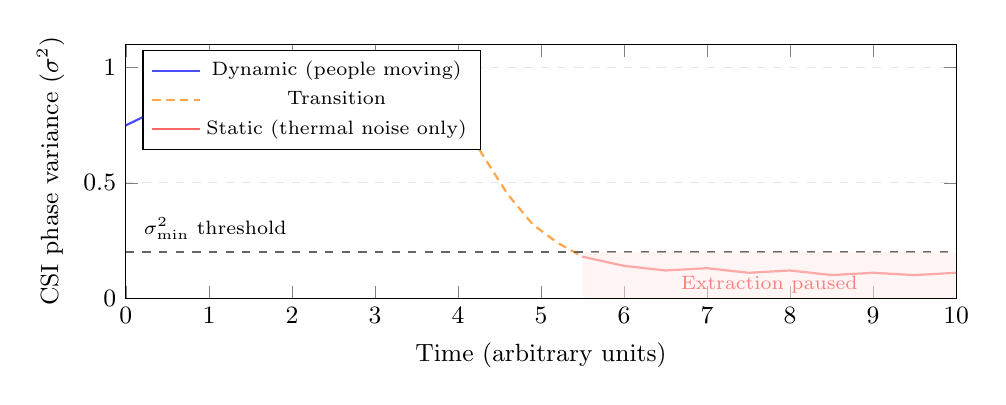
\begin{tikzpicture}
\begin{axis}[
  width=\columnwidth,
  height=4.8cm,
  xlabel={Time (arbitrary units)},
  ylabel={CSI phase variance ($\sigma^2$)},
  xlabel style={font=\small},
  ylabel style={font=\small},
  xticklabel style={font=\small},
  yticklabel style={font=\small},
  xmin=0, xmax=10,
  ymin=0, ymax=1.1,
  ymajorgrids=true,
  grid style={dashed, gray!20},
  legend style={font=\scriptsize, at={(0.02,0.98)}, anchor=north west},
]

% Dynamic environment (high variance, fluctuating)
\addplot[thick, blue!70, mark=none] coordinates {
  (0,0.75) (0.4,0.82) (0.8,0.68) (1.2,0.90) (1.6,0.73) (2.0,0.85)
  (2.4,0.78) (2.8,0.88) (3.2,0.72) (3.6,0.84) (4.0,0.80)
};
\addlegendentry{Dynamic (people moving)}

% Transition (exponential decay)
\addplot[thick, orange!70, mark=none, densely dashed] coordinates {
  (4.0,0.80) (4.3,0.62) (4.6,0.45) (4.9,0.32) (5.2,0.24) (5.5,0.18)
};
\addlegendentry{Transition}

% Static environment (low variance)
\addplot[thick, red!60, mark=none] coordinates {
  (5.5,0.18) (6.0,0.14) (6.5,0.12) (7.0,0.13) (7.5,0.11) (8.0,0.12)
  (8.5,0.10) (9.0,0.11) (9.5,0.10) (10.0,0.11)
};
\addlegendentry{Static (thermal noise only)}

% Threshold line
\draw[dashed, thick, black!60] (axis cs:0, 0.20) -- (axis cs:10, 0.20);
\node[font=\scriptsize, anchor=south west] at (axis cs:0.1, 0.21) {$\sigma^2_{\min}$ threshold};

% Shaded warning zone
\fill[red!8, opacity=0.5] (axis cs:5.5, 0) rectangle (axis cs:10, 0.20);
\node[font=\scriptsize, text=red!50] at (axis cs:7.75, 0.06) {Extraction paused};

\end{axis}
\end{tikzpicture}
\caption{Static environment degradation. When human movement ceases, CSI phase variance drops below $\sigma^2_{\min}$, and the system pauses extraction. In static conditions, only thermal noise provides entropy, at a reduced rate. The variance monitor triggers a switch to fallback sources (QRNG or OS entropy).}
\label{fig:static-degradation}
\end{figure}
